%\documentstyle[10pt,twoside]{article}
%\documentstyle[twoside]{article}
\documentclass[twoside]{article}
\setlength{\oddsidemargin}{0.25 in}
\setlength{\evensidemargin}{-0.25 in}
\setlength{\topmargin}{-0.6 in}
\setlength{\textwidth}{6.5 in}
\setlength{\textheight}{8.5 in}
\setlength{\headsep}{0.75 in}
\setlength{\parindent}{0 in}
\setlength{\parskip}{0.1 in}

\usepackage{graphicx}
\usepackage{url}
\usepackage{enumitem}

%
% The following commands sets up the lecnum (lecture number)
% counter and make various numbering schemes work relative
% to the lecture number.
%
\newcounter{lecnum}
\renewcommand{\thepage}{\thelecnum-\arabic{page}}
\renewcommand{\thesection}{\thelecnum.\arabic{section}}
\renewcommand{\theequation}{\thelecnum.\arabic{equation}}
\renewcommand{\thefigure}{\thelecnum.\arabic{figure}}
\renewcommand{\thetable}{\thelecnum.\arabic{table}}
\newcommand{\dnl}{\mbox{}\par}

%
% The following macro is used to generate the header.
%
\newcommand{\lecture}[4]{
   \pagestyle{myheadings}
   \thispagestyle{plain}
   \newpage
   \setcounter{lecnum}{#1}
   \setcounter{page}{1}
   \noindent
   \begin{center}
   \framebox{
      \vbox{\vspace{2mm}
    \hbox to 6.28in { {\bf CMPSCI~677~~~Operating Systems
                        \hfill Spring 2018} }
       \vspace{4mm}
       \hbox to 6.28in { {\Large \hfill Lecture #1: #2  \hfill} }
       \vspace{2mm}
       \hbox to 6.28in { {\it Lecturer: #3 \hfill Scribe: #4} }
      \vspace{2mm}}
   }
   \end{center}
   \markboth{Lecture #1: #2}{Lecture #1: #2}
   \vspace*{4mm}
}

%
% Convention for citations is authors' initials followed by the year.
% For example, to cite a paper by Leighton and Maggs you would type
% \cite{LM89}, and to cite a paper by Strassen you would type \cite{S69}.
% (To avoid bibliography problems, for now we redefine the \cite command.)
%
\renewcommand{\cite}[1]{[#1]}

% \input{epsf}

%Use this command for a figure; it puts a figure in wherever you want it.
%usage: \fig{NUMBER}{FIGURE-SIZE}{CAPTION}{FILENAME}
\newcommand{\fig}[4]{
            %\vspace{0.2 in}
            \centerline{\includegraphics[scale=#2]{#4}}
            \begin{center}
            Figure \thelecnum.#1:~#3
            \end{center}
    }

% Use these for theorems, lemmas, proofs, etc.
\newtheorem{theorem}{Theorem}[lecnum]
\newtheorem{lemma}[theorem]{Lemma}
\newtheorem{proposition}[theorem]{Proposition}
\newtheorem{claim}[theorem]{Claim}
\newtheorem{corollary}[theorem]{Corollary}
\newtheorem{definition}[theorem]{Definition}
\newenvironment{proof}{{\bf Proof:}}{\hfill\rule{2mm}{2mm}}

% Some useful equation alignment commands, borrowed from TeX
\makeatletter
\def\eqalign#1{\,\vcenter{\openup\jot\m@th
  \ialign{\strut\hfil$\displaystyle{##}$&$\displaystyle{{}##}$\hfil
      \crcr#1\crcr}}\,}
\def\eqalignno#1{\displ@y \tabskip\@centering
  \halign to\displaywidth{\hfil$\displaystyle{##}$\tabskip\z@skip
    &$\displaystyle{{}##}$\hfil\tabskip\@centering
    &\llap{$##$}\tabskip\z@skip\crcr
    #1\crcr}}
\def\leqalignno#1{\displ@y \tabskip\@centering
  \halign to\displaywidth{\hfil$\displaystyle{##}$\tabskip\z@skip
    &$\displaystyle{{}##}$\hfil\tabskip\@centering
    &\kern-\displaywidth\rlap{$##$}\tabskip\displaywidth\crcr
    #1\crcr}}
\makeatother

% **** IF YOU WANT TO DEFINE ADDITIONAL MACROS FOR YOURSELF, PUT THEM HERE:



% Some general latex examples and examples making use of the
% macros follow.

\begin{document}

%FILL IN THE RIGHT INFO.
%\lecture{**LECTURE-NUMBER**}{**DATE**}{**LECTURER**}{**SCRIBE**}
\lecture{14}{March 21}{Prashant Shenoy}{\textbf{Gaurav Anand}}

\section{Overview}
This section covers the following topics:

\begin{description}
  \item[Termination Detection] 
  \item[Leader Election] : Bully Algorithm, Ring Algorithm, Elections in Wireless Networks
  \item[Mutual Exclusion] : Centralized, Decentralized, Distributed algorithms
\end{description}

\section{Distributed Snapshot Algorithm}
We expect a reliable channel such that there is no packet loss and delivery is inorder. TCP gives us those properties out of the box. 
\\
\\
Any process can initiate Snapshot Algorithm. 
\begin{itemize}
\item The initiater will checkpoint it's local state (write memory in disk) and send marker message to every outgoing outgoing channel. 
\item On receiving a marker message the process will checkpoint it's state upon seeing the first marker and send markers on outgoing
channels, also it will save messages on all other incoming channels until another marker is received for that channel.
\end{itemize}

\textbf{Question}: Do we stop executing when they write their state out?\\
\emph{Answer}: While writing memory content we need to ensure that memory does not change. So it will take a pause while writing memory content.

\textbf{Question}: Will this algorithm terminate?\\
\emph{Answer}: If marker message don't get lost then it is guaranteed that algorithm will terminate. We have assumed that messages are not lost and they are delivered inorder.

Multiple snapshots may be in progress so each one is distinguished by tagging the marker with the initiator ID (or sequence number).
This algorithm guarantees consistent cut (distributed snapshot) without the need of synchronization. 


\subsection{Snapshot Algorithm Example}
\begin{figure}[h!]
\centering
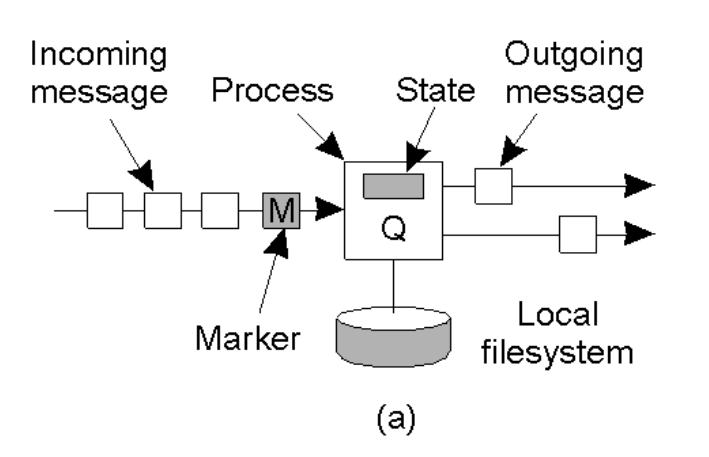
\includegraphics[scale=0.25]{./snapshot_1.png}
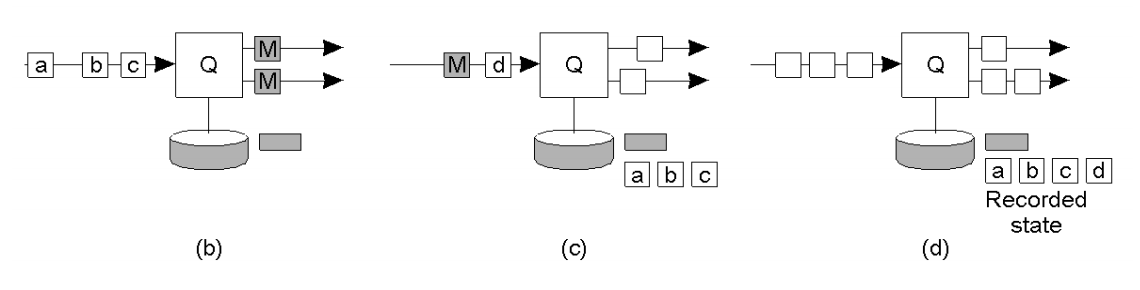
\includegraphics[scale=0.25]{./snapshot_2.png}
\caption{Depiction of Snapshot Algorithm}
\label{fig:bully}
\end{figure} 
\begin{enumerate}[label=(\alph*)]
\item Organization of a process and channels for a distributed snapshot
\item Process Q receives a marker for the first time and records its local state
\item Q records all incoming message
\item Q receives a marker for its incoming channel and finishes recording the state of the incoming channel
\end{enumerate}

\section{Termination Detection}
In a distributed system, the processes might also need to detect when the distributed computation has finished and it should terminate? The entire distributed computation is said to be finished when \emph{every} process in the computation has finished all the work assigned to it and there are no messages in transit. 

The algorithm is similar to the distributed snapshot algorithm. There are two types of marker messages here: \emph{Done} and \emph{Continue}. One of the processes acts as the initiator and sends a query to all of its neighbors asking for their status:\\
\emph{Done}: Done marker message is sent back by the receiver to its predecessor (the process it received the query from) when it has no local job to do and all of its successors have replied with \emph{Done} to it. In addition, the process under consideration should also not have received any outstanding message after it's checked its local job queue, until all of the neighbors reply.\\
\emph{Continue}: Continue is sent back to the predecessor if the process itself has some job to do or if any of its successors have replied back with \emph{Continue} to the process. Continue basically signals that the process, or somebody that process is interacting with(successors), still has some unfinished task.\\
A process sends the marker messages back only after it has received replied from all its successors.

Once the initiator receives \emph{Done} messages from all of its neighbors, it can then broadcast a terminate message asking all the processes to close down.

\section{Leader Election}
Many tasks in distributed systems require one of the processes to act as coordinator. An example of this is the Berkeley algorithm for clock synchronization in which the coordinator has to initiate the synchronization and tell everybody else their offsets. A coordinator can be chosen amongst all processes through leader election. Leaders can be elected manually by the developer(if they know certain machine to be more powerful), or we can have automated leader elections. Automated leader elections are particularly handy in dynamic systems where leaders (coordinators) may quit or crash and a new leader has to be elected. Another example is the unstructured P2P topology which have super-peers elected by a group of peers that wish to have a coordinated process. Two of the automated algorithms are explained below:
\subsection{Bully Algorithm}
The bully algorithm is a simple algorithm, in which we enumerate all the processes running in the system and pick the one with the highest ID as the coordinator (or the one with least load, or best node with best bandwitdh, or some other metric). In this algorithm, each process has a unique id and every process knows the corresponding ID and IP address of every other process. Any process in the system can initiate this algorithm for leader election. Thus, we can have concurrent ongoing elections.

There are three types of messages for this algorithm: \emph{election}, \emph{OK} and \emph{I won}. The algorithm is as follows:
\begin{itemize}
\item{Say a process with id \emph{i} initiates the election.}
\item{It sends \emph{election} messages to all process with id $>$ \emph{i} and awaits OK messages}
\item{If it receives no OK messages, it knows it is the highest id process in the system. It thus sends \emph{I won} messages to all other processes}
\item{If it received OK messages, it knows it is no longer in contention and simply drops out and waits for an \emph{I won} message from some other process}
\item{Any process upon receiving the election message returns an OK to its predecessor and starts an election of its own by sending \emph{election} to higher id processes}
\item{Any process that receives \emph{I won} message treats the sender of that message as coordinator}
\end{itemize}
\begin{figure}[h!]
\centering
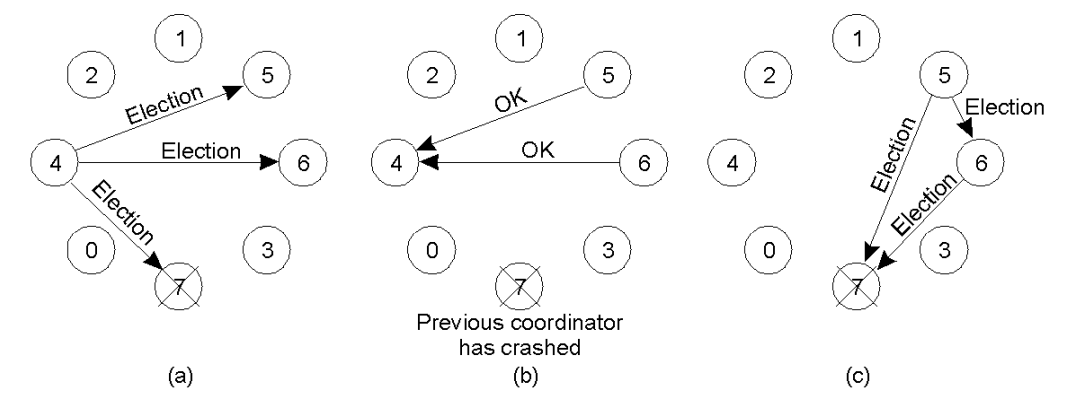
\includegraphics[scale=0.25]{./bully_1.png}
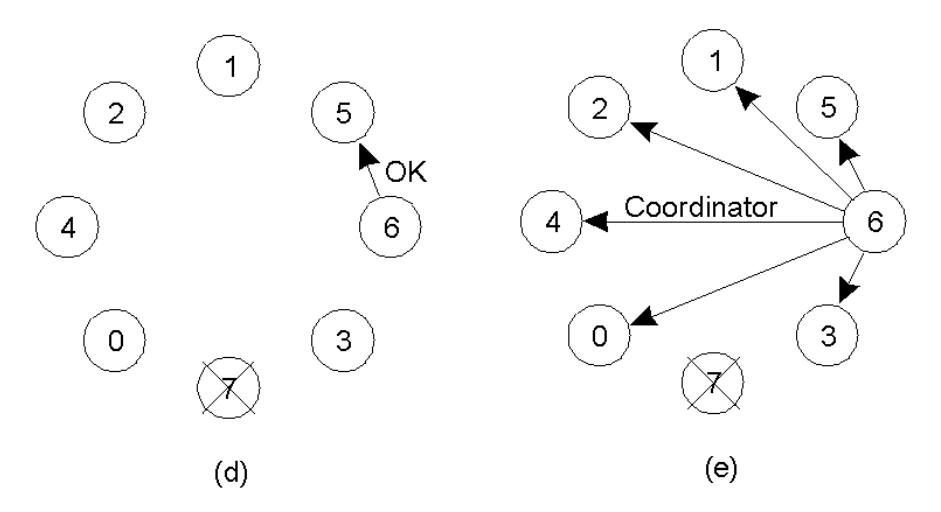
\includegraphics[scale=0.25]{./bully_2.png}
\caption{Depiction of Bully Algorithm}
\label{fig:bully}
\end{figure} 
An example of Bully algorithm is given in Figure \ref{fig:bully}.\\
Communication is assumed to be reliable during leader election. If the communication is unreliable, it may happen that the elected coordinator goes down after it being elected, or a higher id node comes up after the election process. In the former case, any node might start an election process after gauging that the coordinator isn't responding. In the latter case, the higher id process asks its neighbors who is the coordinator. It can then either accept the current coordinator as its own coordinator and continue, or it can start a new election (in which case it will probably be elected as the new coordinator). This algorithm runs in $O(n^2)$ time in the worst case when lowest ID process initiates the election and average case and O(n) time in best case.

\textbf{Question}: What happens when we have a highly dynamic system where processes regularly leave and join (P2P system)?\\
\emph{Answer}: Bully's algorithm is not adequate for all kinds of scenarios. If you have a dynamic system, you might want to take into account the more stable processes (or other metrics) and give them higher ids to have them win elections.

\subsection{Ring Algorithm}
The ring algorithm is similar to Bully's algorithm in the sense that we assume the processes are already ranked through some metric from 1 to n. However, here a process \emph{i} only needs to know the IP addresses of its two neighbors (i+1 and i-1). We want to select the node with the highest id. The algorithm works as follows:
\begin{itemize}
\item{Any node can start circulating the election message. Say process i does so. We can choose to go clockwise or counter-clockwise on the ring. Say we choose clockwise where i+1 occurs after i}
\item{Process i then sends an election message to process i+1}
\item{Anytime a process j($\neq i$) receives an election message, it piggybacks its own id (thus declaring that it is not down) before calling the election message on its successor (j+1)}
\item{Once the message circulates through the ring and comes back to the initiator i, process i knows the list of all nodes that are alive. It simply scans the list and chooses the highest id.}
\item{It lets all other nodes about the new coordinator.}
\end{itemize}
\begin{figure}[h!]
\centering
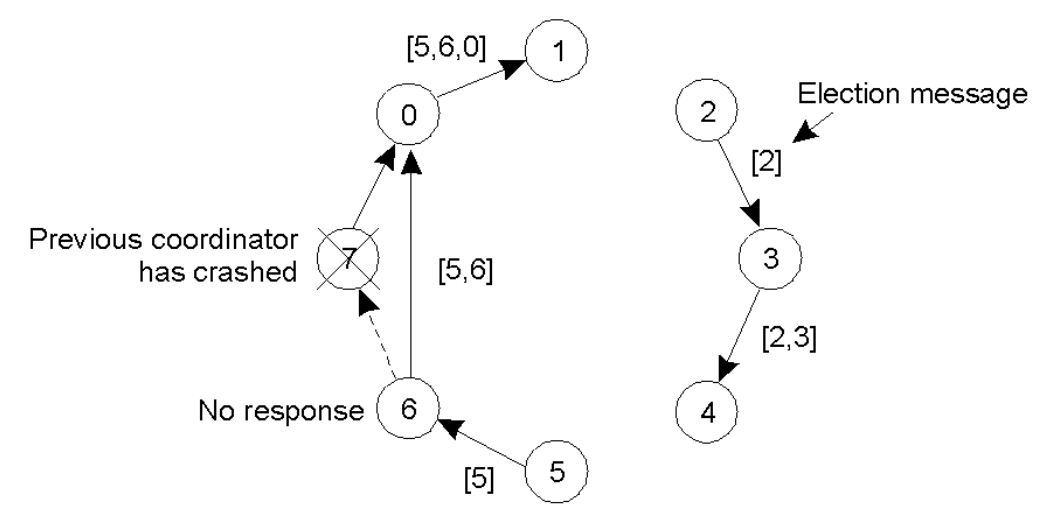
\includegraphics[scale=0.3]{./ring.png}
\caption{Depiction of Ring Algorithm}
\label{fig:ring}
\end{figure} 
An example of Ring algorithm is given in Figure \ref{fig:ring}.

If the neighbor of a process is down, it sequentially polls each successor (neighbor of neighbor) until it finds a live node. For example, in the figure, when 7 is down, 6 passes the election message to 0. Another thing to note is that this requires us to enforce a logical ring topology on the underlying application, i.e. we need to construct a ring topology on top of the whole system just for leader election.

\textbf{Question}: How does 6 know that it has to send message to 0 when 7 is down?\\
\emph{Answer}: Here we can assume that every node not only has information of its neighbors, but neighbors' neighbors as well. In general, in a system where we expect a max of k nodes to go down during the time leader election takes to execute, each node needs to know at least k successive neighbors in either direction. This is still less than what each node needs to know in Bully algorithm.

Ring algorithm always takes 2(n-1) messages to execute. First (n-1) is during the election query and second time to announce the results of the election. It is easy to extend ring algorithm for other metrics like load etc.

\textbf{Question}: How do you know a node is not responding?\\
\emph{Answer}: If it has actually crashed then TCP will fail while setting up socket connection. Otherwise, it can be a slow machine which is taking time. It is a classical problem in distributed systems to distinguish between a slow process and a failed process which is a non-trivial problem. Timeout is not an ideal solution but can be used in practice.

\subsection{Elections in Wireless Networks}
In wireless networks, every node is not in the range of other nodes, and hence even though the whole system is connected, some nodes may not be able to communicate with others. In such a case, the initiator sends a broadcast election message to all its neighbors, and waits for replies from all other nodes. Each node upon receiving such a message broadcasts the election message to all its neighbors. When each such node sends back its response, it attaches its load/capacity and its id on the response. The initiator upon receiving the capacities of all nodes simply picks the one with the highest capacity and declares that node as the leader.

In Skype, a group of peers elect a super-peer. This elected super-peer was required to have adequate capacity to handle all the requests for that group and adequate network bandwidth. The Skype framework also took the stability of a node into account while electing super-peers, since it wanted to avoid the overhead of repeated leader elections.

\section{Mutual Exclusion}
Everytime we wish to access a shared data structure or critical section in a distributed system, we need to guard it with a lock. A lock is acquired before the data structure is accessed, and once the transaction has completed, the lock is released.

\subsection{Centralized Mutual Exclusion}
In this case, locking and unlocking coordination is done by a master process. All processes are numbered 1 to n. We run leader election to pick the coordinator.

Now, if any process in the system wants to acquire a lock, it has to first send a lock acquire request to the coordinator. Once it sends this request, it blocks execution and awaits reply until it acquires the lock. The coordinator maintains a queue for each data structure of lock requests. Upon receiving such a request, if the queue is empty, it grants the lock and sends the message, otherwise it adds the request to the queue. The requestor process upon receiving the lock executes the transaction, and then sends a release message to the coordinator. The coordinator upon receipt of such a message, removes the next request from the corresponding queue and grants that process the lock.

\begin{figure}[h!]
\centering
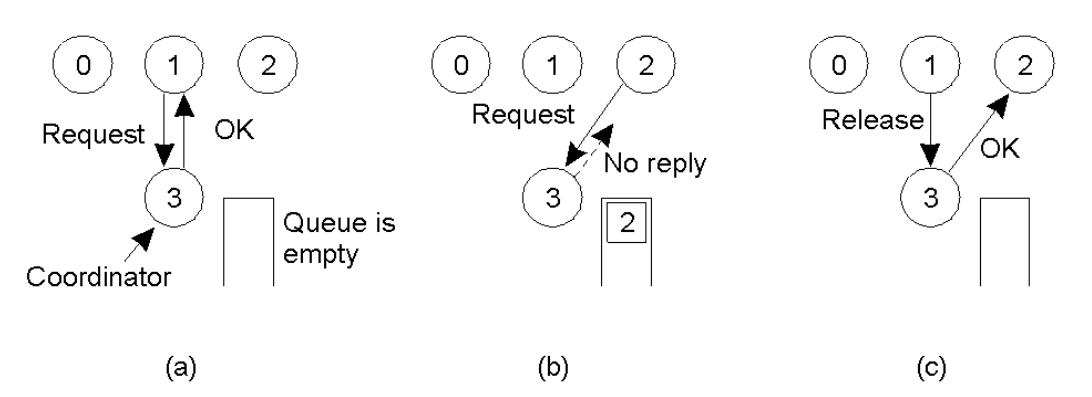
\includegraphics[scale=0.33]{./centralized.png}
\caption{Depiction of Centralized Mutual Exclusion Algorithm}
\label{fig:centralized}
\end{figure} 
An example of the algorithm is given in Figure \ref{fig:centralized}.

There are two major issues with this algorithm, related to failures. When coordinator process goes down while one of the processes is waiting on a response to a lock request, it leads to inconsistency. The new coordinator that is elected (or reboots) might not know that the earlier process is still waiting for a response. This issue can be tackled by maintaining persistent data on disk whenever a queue of the coordinator is altered. Even if the process crashes, we can read the file and persist the state of the locks on storage and recover the process.

The harder problem occurs when one of the client process crashes while it is holding the lock (during one of its transactions). In such a case, coordinator is just waiting for the lock to be released while the other process has gone down. We cannot use timeout in this case, because usually transactions take arbitrary amount of time to go through. All other processes that are waiting on that lock are also blocked forever. Even if the coordinator somehow knew that the client process has crashed, it may not always be advisable to take the lock forcibly back because the client process may eventually reboot and think it has the lock and continue its transaction. This causes inconsistency. This is a thorny problem which does not have any neat solution. This limits the practicality of such an centralized algorithm.

\subsection{Decentralized Algorithm}
Decentralized algorithms use voting to figure out which lock requests to grant. In this scenario, each process has an extra thread called the coordinator thread which deals with all the incoming locking requests. Essentially, every process keeps a track of who has the lock, and for a new process to acquire a new lock, it has to be granted an \emph{OK} or go ahead vote from the strict majority of the processes. Here, majority means more than half the total number of nodes (live or not) in the system. Thus, if any process wishes to acquire a lock, it requests it from all other processes and if the majority of them tell it to acquire the lock, it goes ahead and does so. Majority guarantees that a lock is not granted twice. Upon the receipt of the vote, the other processes are also told that a lock has been acquired and thus, the processes hold up any other lock request. Once a process is done with the transaction, it broadcasts to every other process that it has released the lock.

This solves the problem of coordinator failure because if some nodes go down, we can deal with it so long as the majority agrees that whether the lock is in use or not. Client crashes are still a problem here.

\subsection{Distributed Algorithm}
This algorithm, developed by Ricart and Agrawala needs 2(n-1) messages and is based on Lamport's clock and total ordering of events to decide on granting locks. Basically, after the clocks are synchronized, the process that asked for the lock first gets it. The initiator sends request messages to all n-1 processes stamped with its id and the timestamp of its request. It then waits for replies from \emph{all} other processes.

Any other process upon receiving such a request either sends reply if it does not want the lock for itself, or is already in the transaction phase (in which case it doesn't send any reply and the initiator has to wait), or it itself wants to acquire the same lock in which case it compares its own request timestamp with that of the incoming request. The one with the lower timestamp gets the lock first.

\begin{itemize}
\item Process k enters critical section as follows
  \begin{itemize}
    \item Generate new time stamp $TS_k$ = $TS_{k+1}$
    \item Send request(k,$TS_k$) all other n-1 processes
    \item Wait until reply(j) received from all other processes
    \item Enter critical section
  \end{itemize}
\item Upon receiving a request message, process j
  \begin{itemize}
    \item Sends reply if no contention
    \item If already in critical section, does not reply, queue request
    \item If wants to enter, compare $TS_j$ with $TS_k$ and send reply if $TS_k<TS_j$ , else queue (recall: total ordering based on multicast)
  \end{itemize}
\end{itemize}

Fully decentralized but there are n points of \textbf{failure}, which is worse than a centralized one.

\subsection{Token Ring Algorithm}
Actual topology is not a ring but for locking purpose there is a logical ring. And process only talk to neighbor processes. A process with the token has the lock at that time. To acquire the lock one needs to wait. The token is circulated through the logical ring. No method is there to request token, the process needs to wait to get a lock.

In this algorithm one problem is loss of token, regenerating token is non-trivial, can not use timeout strategy. 

\end{document}
